\documentclass[conference]{IEEEtran}
\usepackage[T1]{fontenc}
\usepackage{graphicx}
\usepackage{booktabs}
\usepackage{amsmath,amssymb}
\usepackage{xcolor}
\usepackage{tikz}
\usetikzlibrary{positioning,arrows.meta,fit,calc}
\usepackage[hidelinks]{hyperref}
\usepackage{cite}
\usepackage{url}

\newcommand{\Tacc}{T_{\mathrm{acc}}}

\begin{document}

\title{When Does Shared-Bus Arbitration Fail to Protect Streaming Sensors During TinyML Inference?\\
\large A SystemC Failure-Map Study on a RISC-V Virtual Prototype}

\author{\IEEEauthorblockN{Abdelrahman Youssef}
\IEEEauthorblockA{Computer Engineering Department\\
King Fahd University of Petroleum and Minerals (KFUPM), Saudi Arabia\\
COE 407/661 System on Chip --- term paper}}

\maketitle

\begin{abstract}
A TinyML system-on-chip shares one interconnect between three kinds of traffic: a CPU that runs a hard real-time control loop, a streaming sensor whose small FIFO is drained by DMA, and a DNN accelerator whose DMA moves weights and activations. This paper builds a request/grant bus arbiter in SystemC/TLM-2.0 inside the RISC-V VP++ virtual prototype, with a STONNE-timed accelerator running the MLPerf Tiny DS-CNN network, and maps where five arbitration policy variants---round-robin, two fixed priorities, a buffer-status priority and a budget-with-fragmentation regulator---stop meeting three limits fixed in advance from datasheets and the real-time literature: no sensor overflow within a FIFO of 8 (strict) or 1280 (relaxed) samples, no missed control-loop deadline, and at most 10\,\% inference delay. A sufficient FIFO bound is derived and holds at all 100 points where it applies (measured minimum 0.50--1.00 of the bound, 229 vs.\ 230 samples at the tightest point). Over 240 configurations and 1{,}036 simulations, the four non-throttling policies give minimum FIFO depths within one sample of each other: on a bus whose bursts cannot be interrupted, the sensor always waits for one in-flight DNN burst whatever the grant order. The outcome is decided instead by the DNN burst length (1024-byte bursts make the control loop miss 17 of 80 deadlines under every policy; 256-byte bursts meet it at 8\,\% inference cost), by the sensor's drain threshold, and by the 10-cycle setup of every burst. All limits are met with an 8-sample FIFO up to 3.2\,MB/s, only with a $\approx$145-sample FIFO at 32\,MB/s, and not at 100\,MB/s, where the sensor's bus share alone exceeds the delay margin. Under this bus model, no feasible point exists where every established policy fails, which locates a possible research target in settings where grant order does matter.
\end{abstract}

\begin{IEEEkeywords}
bus arbitration, DMA, streaming sensor, FIFO sizing, real-time, TinyML, DNN accelerator, SystemC, TLM-2.0, RISC-V virtual prototype
\end{IEEEkeywords}

\section{Introduction}
Microcontroller-class SoCs now run DNN inference next to the sensor that feeds them: keyword spotting next to a microphone, vision next to a camera interface, and, at the high end, signal classification next to an RF analog-to-digital converter. In such a chip the accelerator's DMA, the sensor's DMA and the CPU share one interconnect. A sensor that cannot get the bus in time overflows its FIFO and loses samples; a CPU control loop that waits too long for the bus misses its deadline; and every cycle given to the sensor or the CPU delays the inference. The designer chooses three things that decide this trade-off: the arbitration policy, the DMA burst length, and the FIFO size with its drain threshold.

This paper measures, in simulation, where standard arbitration policies stop protecting a streaming sensor and a CPU deadline while a DNN runs, and what that protection costs in inference time. It makes four technical contributions:
\begin{itemize}
\item a request/grant shared-bus model in SystemC/TLM-2.0 with three masters, five policy variants and a handover cost on ownership change, integrated into the RISC-V VP++ virtual prototype with a STONNE-timed DNN accelerator (Section~\ref{sec:model});
\item a sufficient FIFO-depth bound for a sensor whose DMA drains $\theta$ samples per burst, with its proof, used as a one-sided check of the simulator (Section~\ref{sec:bound});
\item acceptance limits fixed before any sweep from datasheets and the real-time literature (Section~\ref{sec:limits});
\item a failure map over policy, DNN burst length, sensor rate, drain threshold and FIFO depth, with the exact minimum FIFO depth found by bisection, and a test of whether any feasible point defeats every policy (Section~\ref{sec:results}).
\end{itemize}
The study is a case study under an explicitly stated bus model, not a hardware timing guarantee. All code, scripts and the 1{,}036 result files are public.\footnote{\url{https://github.com/AbdelRahmanAtef1911/soc-accel-project}}

\section{Background and Related Work}\label{sec:related}
\textbf{Accelerator contention on shared buses.} Restuccia et al.\ restore fairness in AXI round-robin arbiters~\cite{restuccia19}, model bus contention of FPGA accelerators analytically~\cite{restuccia20}, bound memory access times with several accelerators~\cite{restuccia23} and make DNN acceleration time-predictable~\cite{restuccia21}. Brilli et al.\ measure CPU/accelerator memory interference on FPGA SoCs~\cite{brilli}, and Oliveira et al.\ study shared-resource contention and timeliness on low-end MCUs~\cite{oliveira}. Pujol et al.\ discuss the limits of AXI4 time predictability~\cite{pujol}.

\textbf{Arbitration and regulation.} Real-time interconnects include AXI-IC$^{RT}$~\cite{axiicrt}, buffer-aware arbitration~\cite{roh} and bandwidth-control arbitration evaluated in SystemC~\cite{sudo}. AXI-REALM regulates traffic per manager with budgets and burst fragmentation~\cite{axirealm}; Carfield uses a similar traffic shaper in silicon~\cite{carfield}, and Benz's thesis covers real-time DMA and sensor I/O~\cite{benz}. Deadline-aware schedulers prioritise accelerator traffic by progress~\cite{squash,dash} or arbitrate a shared last-level cache~\cite{flash}; on phones, NPU traffic priority hurts foreground work~\cite{sereno}.

\textbf{DNN timing under contention.} Execution time and WCET of CNNs under memory contention are predicted or bounded for FPGA DPUs~\cite{tpds,express,rtdpu}; multiple DNNs are scheduled on MCUs with external memory~\cite{rtmdm}; contention-aware co-scheduling~\cite{haxconn} and data-movement-aware accelerator scheduling~\cite{relief} reduce interference; a compile-time schedule of shared-memory accesses gives a time-triggered alternative~\cite{kirschner}.

\textbf{Modelling.} STONNE gives cycle-level DNN accelerator timing~\cite{stonne}; the RISC-V VP and VP++ are SystemC virtual prototypes~\cite{rvvp,vppp}; loosely-timed SystemC DNN models with memory contention are shown in~\cite{arasteh}. The workload is DS-CNN from MLPerf Tiny~\cite{mlperftiny}; DORY~\cite{dory} and $\mu$NPU benchmarking~\cite{unpu} show that data movement matters on MCU-class accelerators.

This paper uses the mechanisms above as baselines---round-robin, fixed priority, a buffer-status priority inspired by~\cite{roh}, and a budget with fragmentation inspired by~\cite{axirealm,carfield}---and asks where, together, they meet a streaming sensor's FIFO limit, a hard CPU deadline and an inference-delay margin. The two derived variants keep only the core mechanism of the cited designs; AXI-REALM, for example, also has monitoring and further regulation that are not modelled.

\section{System and Bus Model}\label{sec:model}
\begin{figure}[t]
\centering
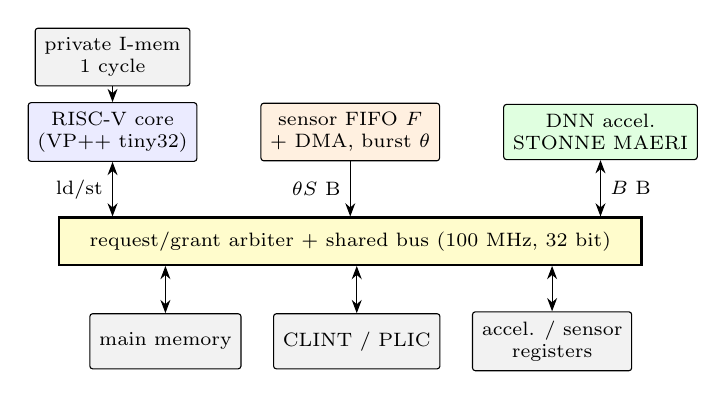
\begin{tikzpicture}[font=\scriptsize, node distance=4mm,
  blk/.style={draw, rounded corners=1pt, minimum height=7mm, minimum width=17mm, align=center, fill=#1},
  blk/.default=white, >=Stealth]
\node[blk=blue!8] (cpu) {RISC-V core\\(VP++ tiny32)};
\node[blk=gray!10, above=2mm of cpu] (imem) {private I-mem\\1 cycle};
\node[blk=orange!12, right=8mm of cpu] (sen) {sensor FIFO $F$\\+ DMA, burst $\theta$};
\node[blk=green!12, right=8mm of sen] (acc) {DNN accel.\\STONNE MAERI};
\node[draw, thick, fill=yellow!20, minimum width=74mm, minimum height=6mm, below=7mm of sen] (bus)
  {request/grant arbiter + shared bus (100 MHz, 32 bit)};
\node[blk=gray!10, below=6mm of bus.south west, anchor=north west, xshift=4mm] (mem) {main memory};
\node[blk=gray!10, right=4mm of mem] (clint) {CLINT / PLIC};
\node[blk=gray!10, right=4mm of clint] (regs) {accel. / sensor\\registers};
\draw[->] (imem) -- (cpu);
\draw[<->] (cpu) -- (cpu|-bus.north) node[midway,left]{ld/st};
\draw[->] (sen) -- (sen|-bus.north) node[midway,left]{$\theta S$ B};
\draw[<->] (acc) -- (acc|-bus.north) node[midway,right]{$B$ B};
\draw[<->] (mem.north) -- (mem.north|-bus.south);
\draw[<->] (clint.north) -- (clint.north|-bus.south);
\draw[<->] (regs.north) -- (regs.north|-bus.south);
\end{tikzpicture}
\caption{Modelled SoC. The CPU fetches instructions from a private memory; its loads and stores, the sensor DMA and the DNN DMA compete for one shared bus.}
\label{fig:soc}
\end{figure}

\textbf{Platform.} The platform (Fig.~\ref{fig:soc}) is the RISC-V VP++ \emph{tiny32} core at 100\,MHz~\cite{vppp} with a memory-mapped DNN accelerator modelled in SystemC/TLM-2.0, whose compute time comes from STONNE (MAERI, 256 multipliers, distribution bandwidth 256)~\cite{stonne}. The accelerator runs convolutions natively, tiles the layer (4 tiles) and double-buffers DMA and compute; it signals completion by interrupt and the CPU sleeps (WFI) meanwhile. CPU instruction fetches come from a private 1-cycle memory (an instruction TCM); the CPU's loads and stores---stack, filter state, peripheral registers---use the shared bus. This choice is stated because it matters: with fetches on the bus the CPU contends on every instruction, and with a data TCM it would barely contend at all.

\textbf{Bus.} One 32-bit bus at 100\,MHz connects all masters to one memory. A request/grant arbiter grants the bus only when it is free; each master has at most one outstanding request; a granted burst cannot be interrupted (no split transactions). A burst of $b$ bytes holds the bus for
\begin{equation}
c(b) = 10 + \lceil b/4 \rceil \text{ cycles},\label{eq:burst}
\end{equation}
a CPU access for one cycle. When ownership changes, the next tenure starts $a=1$ cycle later (handover); consecutive grants to the same master pay nothing. Requests made in the same simulated instant are collected for one delta cycle before the arbiter decides, so the policy, not the SystemC process order, resolves ties. The CPU port synchronises the core's local time before every access and performs the access only after the grant, so, e.g., an accelerator START write takes effect inside the CPU's tenure.

\textbf{Masters.} (i) The CPU runs a control task released every 62\,$\mu$s by the CLINT timer (16-tap FIR; deadline = next release) and sleeps in between. (ii) The DNN DMA moves bursts of $B\in\{64,256,1024\}$\,bytes. (iii) The sensor delivers one $S=4$-byte sample every $1/R$ into a FIFO of $F$ samples; a sample arriving at a full FIFO is dropped. Its DMA requests the bus when the FIFO holds $\theta$ samples, moves exactly $\theta$ samples per burst, and frees them when the burst completes (a conservative removal rule). No rule reads $F$, so as long as nothing overflows, request times do not depend on $F$.

\textbf{Policy variants.} (1) round-robin; (2) sensor-first fixed priority (sensor$>$CPU$>$DNN); (3) CPU-first (CPU$>$sensor$>$DNN); (4) buffer-status: the sensor competes round-robin until its FIFO holds $2\theta$ samples, then has top priority (simplified, after~\cite{roh}); (5) budget with fragmentation: DNN transfers are split into 64-byte fragments, and the DNN may be granted at most $X$ bytes per aligned window of 1000 cycles, $X=\rho\cdot 4000$ with $\rho\in\{0.25,0.5\}$; eligible requests are served round-robin (simplified, after~\cite{axirealm,carfield}).

\textbf{Workload and measurement.} After a warm-up of 16 control periods, one DS-CNN inference (10 layers, timing-only tensors, no feature extraction) is released; $\Tacc$ runs from that release to the end of the last layer, and its deadline is $T_{\mathrm{inf}}=5$\,ms. Overflows, control-task misses and bus occupancy are counted in the window $[$release, release$+T_{\mathrm{inf}})$. MLPerf Tiny supplies only the network; the sensor, CPU and bus scenario is this paper's model, so the results are not MLPerf Tiny results~\cite{mlcommons}. The DNN delay $\Delta\Tacc$ is measured against the no-sensor run at the same $B$ without throttling, so the throttling of variant~5 counts as a protection cost.

\section{A Sufficient FIFO Bound}\label{sec:bound}
Under sensor-first priority no master outranks the sensor, so after requesting it waits at most for one lower-priority tenure already in progress plus the handover. With blocking $\beta = c(B)$ cycles and its own burst $\sigma = c(\theta S)$, the worst time from request to burst completion is $L=\beta+a+\sigma$ cycles. A periodic source delivers at most $\lceil R L/f\rceil$ samples in any half-open interval of $L/f$ seconds.

\textbf{Proposition.} No sample overflows if
\begin{align}
\text{(C1)}\quad & F \ge \theta + \lceil R L / f \rceil, \label{eq:c1}\\
\text{(C2)}\quad & \lceil R L / f \rceil \le \theta. \label{eq:c2}
\end{align}
\emph{Proof.} By induction over drain rounds. A request is raised when occupancy reaches $\theta$. Until its burst completes at most $\lceil RL/f\rceil$ samples arrive, so the peak occupancy is $\theta+\lceil RL/f\rceil\le F$ by (C1) and no arriving sample finds the FIFO full. At completion $\theta$ samples leave, so at most $\lceil RL/f\rceil\le\theta$ remain by (C2); the next request is again raised at occupancy $\theta$, and the argument repeats. $\square$

For round-robin, $\beta$ becomes one tenure of each other master plus a handover, $\beta_{RR}=c(B)+1+a$. No bound is claimed for CPU-first, whose CPU demand the model does not bound. The bound is sufficient, not tight, and is used one-sidedly: every simulated point that satisfies (C1)--(C2) must show zero overflows.

\textbf{Bus-overhead estimate.} Because the double-buffered DS-CNN is largely bus-bound, a sensor that takes a bus share $s=(R/\theta)(c(\theta S)+a)/f$ delays it by roughly $s/(1-s)$. The smallest share reachable within a FIFO limit uses the largest allowed $\theta$; where even that share exceeds the delay margin, no arbiter can meet the margin, and the point is excluded from the gap test as \emph{bandwidth-infeasible}. This is an estimate, not a bound, and is checked against the simulations below.

\section{Acceptance Limits}\label{sec:limits}
The limits were fixed before the sweeps (Table~\ref{tab:limits}). The sensor limit follows from the camera-interface note that a FIFO has no overrun protection when the bus cannot keep up~\cite{an5020}. The strict FIFO size is typical of on-chip peripheral FIFOs: an 8-word audio FIFO~\cite{rm0432}, an 8-sample ADC FIFO~\cite{rp2040} and a 4-word camera FIFO~\cite{an5020}; the relaxed size is the 5120-byte camera-pipeline FIFO reported for a recent MCU~\cite{stforum} (a forum report). The control task is hard real-time~\cite{buttazzo}. The 10\,\% delay margin has no standard value in the literature; it is a stated design choice, and the gap test is repeated at 5\,\% and 25\,\%.

\begin{table}[t]
\caption{Acceptance limits, fixed before the sweeps}
\label{tab:limits}
\centering\footnotesize
\begin{tabular}{@{}ll@{}}
\toprule
Limit & Value \\ \midrule
Sensor data & zero FIFO overflows in the window \\
FIFO size & strict $F\le 8$ samples; relaxed $F\le 1280$ samples \\
CPU & zero late or lost releases of the 62\,$\mu$s task \\
DNN deadline & $\Tacc \le T_{\mathrm{inf}} = 5$\,ms \\
DNN delay & $\Delta\Tacc \le 10\,\%$ (also 5\,\% and 25\,\%) \\ \bottomrule
\end{tabular}
\end{table}

\section{Validation}\label{sec:validation}
\textbf{Unit tests.} Seven tests drive the arbiter with stub masters. Each variant grants three simultaneous requests in its documented order. Under sensor-first priority with 1024-byte DNN bursts ($c=266$ cycles), the sensor's worst wait is 267 cycles $=\beta+a$, and under round-robin 268 cycles against a bound of 270. With three saturating masters and equal 64-byte requests, round-robin grants 2470/2469/2469 times; with unequal tenures it still equalises grants, and each master's busy share equals its tenure divided by the sum of tenures plus handovers. Fixed priority starves the lower masters under saturation. The budget variant grants exactly 960 of 1000 allowed bytes in every aligned window. In 13{,}794 alternating tenures, the 13{,}793 handovers equal the ownership changes, and no tenures overlap.

\textbf{Regression.} With handover $a=0$ the request/grant bus reproduces the earlier accelerator testbench cycle counts exactly; with $a=1$ every job is exactly one cycle longer---the one ownership change after the CPU's START write. A CPU-only benchmark run (48 layers in software) is identical to the earlier result, and the earlier bus model is unchanged.

\textbf{Bound and monotonicity.} Over all sweeps, the 50 sensor-first and 50 round-robin points that satisfy (C2) all meet $F_{\min}\le F_{\mathrm{suf}}$, with $F_{\min}/F_{\mathrm{suf}}$ between 0.50 and 1.00. At 100\,MB/s, $B=1024$, $\theta=128$, the bound gives 230 samples; the measured minimum is 229 and the sensor's worst wait is 267 cycles. Runs at $F_{\min}$ and at $F=512$ give identical window results at all six sampled points, confirming that overflow-freedom is monotonic in $F$, so $F_{\min}$ can be found by bisection.

\section{Experiments and Results}\label{sec:results}
\textbf{Sweeps.} Stage A (124 runs) covered variants 1--4, $B\in\{64,1024\}$, five sensor rates from 32\,kB/s to 100\,MB/s and three depths, with $\theta$ set to the smallest power of two that satisfies (C2). It showed that this choice of $\theta$ minimises the FIFO but maximises the per-burst overhead. Stage B (240 configurations, 912 runs) therefore sweeps $\theta$ in powers of two up to 128, adds $B=256$ and variant~5, and finds the exact minimum depth $F_{\min}$ by integer bisection on $[\theta,512]$; the CPU and DNN results of the passing run hold for every $F\ge F_{\min}$.

\begin{table}[t]
\caption{No-sensor runs (identical for variants 1--4)}
\label{tab:base}
\centering\footnotesize
\begin{tabular}{@{}lrrr@{}}
\toprule
DNN setting & $\Tacc$ (cycles) & control task late/lost & worst resp. (cyc) \\ \midrule
$B=64$ & 205{,}163 & 0/80 & 1{,}207 \\
$B=256$ & 158{,}738 & 0/80 & 3{,}212 \\
$B=1024$ & 146{,}389 & 17/80 & 10{,}134 \\
budget, $\rho=0.5$ & 234{,}179 & 0/80 & 1{,}182 \\
budget, $\rho=0.25$ & 434{,}070 & 0/80 & 722 \\ \bottomrule
\end{tabular}
\end{table}

\textbf{The burst length decides the CPU deadline.} Table~\ref{tab:base} shows the runs without a sensor. With 1024-byte bursts the control task misses 17 of 80 releases under \emph{every} policy, CPU-first included: each of its $\approx$100 loads and stores may wait for an in-flight 266-cycle burst, and its worst response (10{,}134 cycles) exceeds the 6{,}200-cycle period. 256-byte bursts keep the worst response at 3{,}212 cycles for 8\,\% more inference time than 1024-byte bursts; 64-byte bursts cost 40\,\%. The budget variant protects the CPU at $B=1024$ but throttles the DNN by 60\,\% ($\rho=0.5$) to 197\,\% ($\rho=0.25$).

\begin{figure*}[t]
\centering
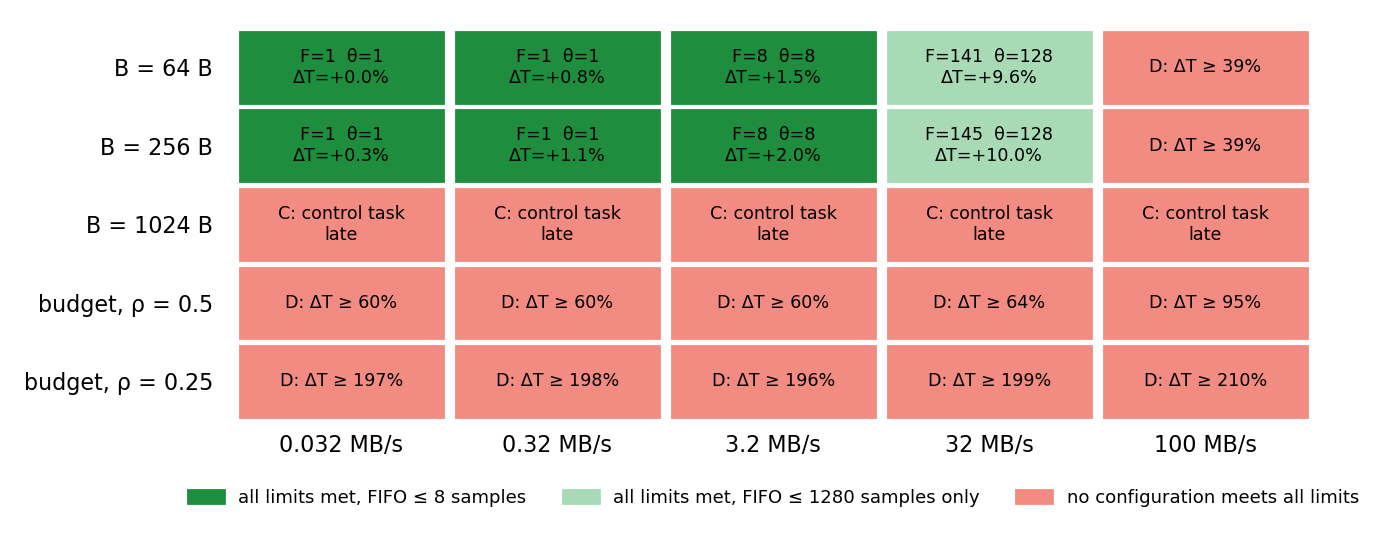
\includegraphics[width=0.78\textwidth]{figures/fig1_failure_map.png}
\caption{Failure map (delay margin 10\,\%). For each DNN setting and sensor rate, the best configuration over variants 1--4 and $\theta$ (variants 1--4 behave alike, Table~\ref{tab:inv}); text gives its $F_{\min}$, $\theta$ and $\Delta\Tacc$, or the limit that no configuration meets (C: control task, D: DNN delay).}
\label{fig:map}
\end{figure*}

\textbf{Failure map.} Fig.~\ref{fig:map} summarises the map. All limits are met with the strict 8-sample FIFO up to 3.2\,MB/s, with 64- or 256-byte bursts and $\theta=8$ at 3.2\,MB/s ($\Delta\Tacc$ 1.5--2.0\,\%). At 32\,MB/s only the relaxed FIFO works, with $\theta=128$ and $F_{\min}=141$--145 at $\Delta\Tacc\approx 10\,\%$. At 100\,MB/s no configuration meets the margin: even with $\theta=128$ the sensor needs about 27\,\% of the bus. 1024-byte bursts fail the control task everywhere, and the budget variants fail the delay margin everywhere.

\begin{figure*}[t]
\centering
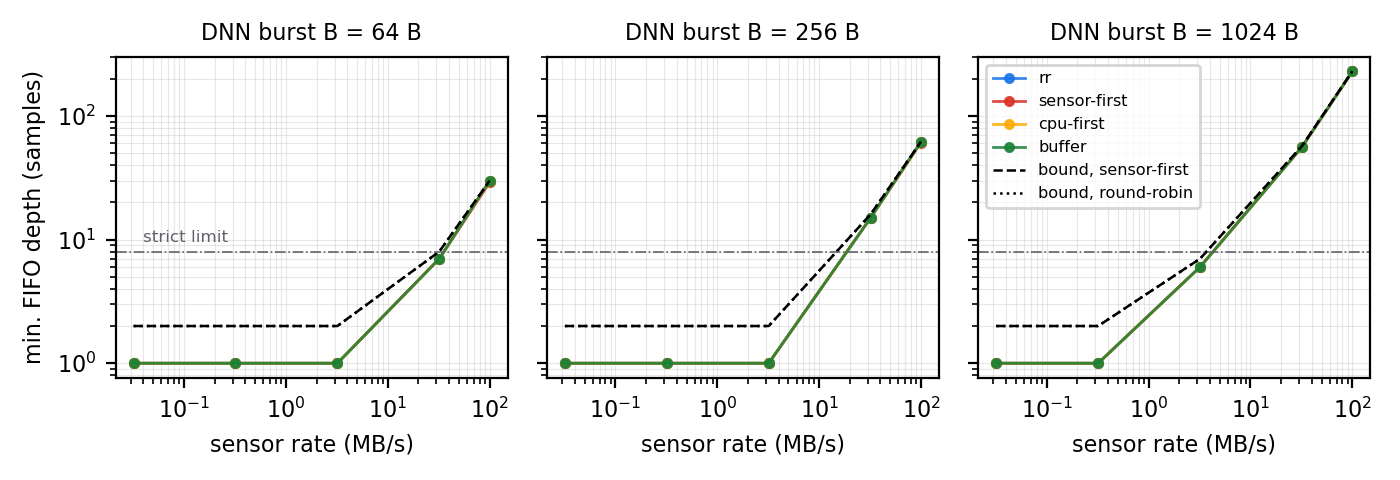
\includegraphics[width=0.78\textwidth]{figures/fig2_min_fifo.png}
\caption{Exact minimum FIFO depth vs.\ sensor rate ($\theta$ = smallest value meeting (C2)). The four variants overlap; dashed and dotted lines are the sufficient bounds for sensor-first and round-robin.}
\label{fig:fifo}
\end{figure*}

\begin{table}[t]
\caption{Policy invariance over 50 (burst, rate, $\theta$) points, variants 1--4}
\label{tab:inv}
\centering\footnotesize
\begin{tabular}{@{}lr@{}}
\toprule
Quantity & largest spread across policies \\ \midrule
minimum FIFO depth $F_{\min}$ & 1 sample (3.3\,\%) \\
DNN delay $\Delta\Tacc$ & 2.6 percentage points \\
CPU deadline outcome & differs at 3 of 50 points \\ \bottomrule
\end{tabular}
\end{table}

\textbf{Grant order hardly matters.} Fig.~\ref{fig:fifo} and Table~\ref{tab:inv} show the central result: the four non-throttling variants give minimum FIFO depths within one sample of each other at every point. On a bus whose bursts cannot be interrupted, the sensor's worst wait is one in-flight DNN burst whatever the order---the bound's $\beta$---and the CPU's one-cycle accesses are the only thing the order changes. Round-robin adds one CPU access to that wait; sensor-first removes it. The DNN delay is likewise set by how much of the bus the others use, not by when they use it, because the arbiter is work-conserving.

\begin{figure*}[t]
\centering
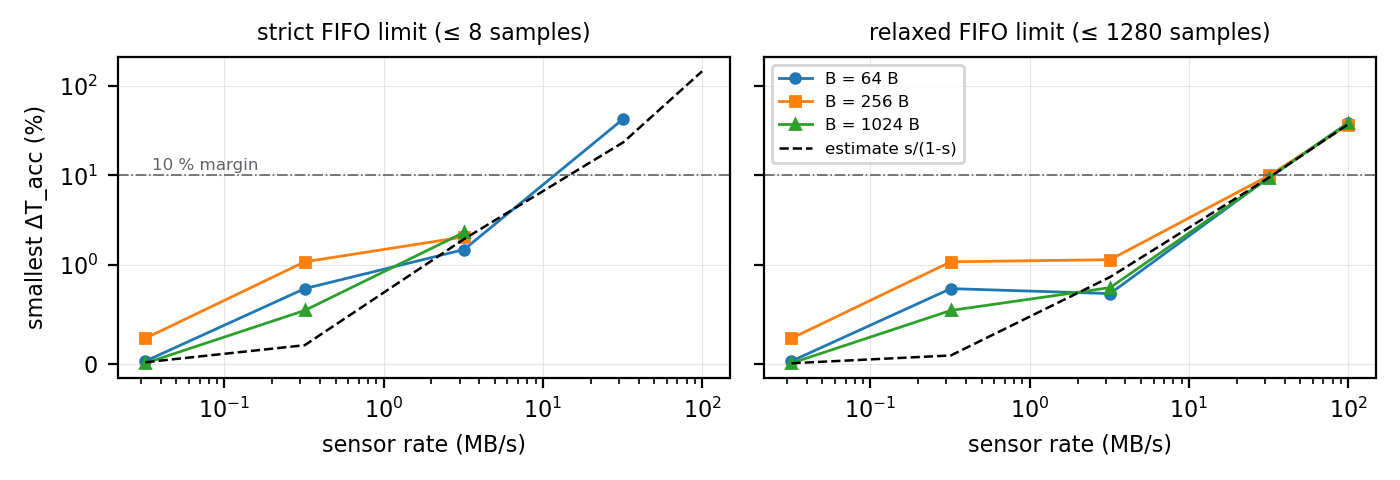
\includegraphics[width=0.78\textwidth]{figures/fig3_delay.png}
\caption{Smallest DNN delay reachable within each FIFO limit (over variants 1--4 and $\theta$), with the bus-overhead estimate $s/(1-s)$ at the largest $\theta$ the limit allows. $B=1024$ points miss the CPU deadline (Fig.~\ref{fig:map}).}
\label{fig:delay}
\end{figure*}

\textbf{The delay follows the sensor's bus share.} Fig.~\ref{fig:delay} compares the smallest reachable delay with the overhead estimate. The estimate tracks the simulations from 3.2\,MB/s upward, and no simulated configuration within a FIFO limit meets the delay margin where the estimate says it cannot (0 violations at all three margins and both FIFO limits). With the strict FIFO, the 10-cycle setup of 32-byte sensor bursts already costs about 19\,\% of the bus at 32\,MB/s.

\begin{figure*}[t]
\centering
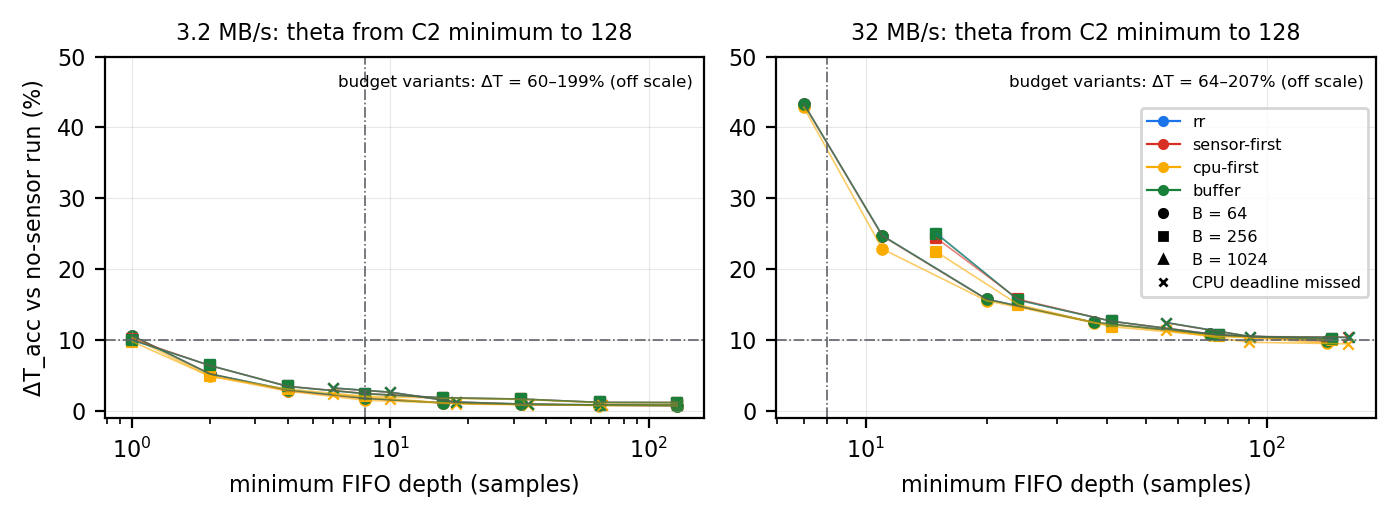
\includegraphics[width=0.78\textwidth]{figures/fig4_tradeoff.png}
\caption{Trade-off between minimum FIFO depth and DNN delay as $\theta$ grows (one line per policy and burst length; $\times$: CPU deadline missed). Dash-dotted lines: strict FIFO limit and 10\,\% margin.}
\label{fig:trade}
\end{figure*}

\textbf{The drain threshold trades FIFO for overhead.} Fig.~\ref{fig:trade} shows the trade-off that $\theta$ controls. At 3.2\,MB/s, $\theta=1$ needs a one-sample FIFO but costs about 10\,\%, while $\theta=8$ fits the strict limit at 1.5--2.4\,\%. At 32\,MB/s the curve crosses the 10\,\% margin only near $F\approx 140$; inside the strict limit the best point is $\theta=4$, $F_{\min}=7$, at a 43\,\% delay. Lines of different policies lie on top of each other.

\textbf{Research-gap test.} The plan asked whether a feasible point exists where every established policy fails to meet all limits together. Excluding points that are bandwidth-infeasible by the estimate, the answer is no for both FIFO limits at 5\,\% and 10\,\% margins and for the relaxed FIFO at 25\,\%. One candidate remains: 32\,MB/s with the strict FIFO and a 25\,\% margin. There $\theta=8$ would meet the margin ($\Delta\Tacc$ 22--25\,\%) but needs $F_{\min}=11$--15, because samples keep arriving during the sensor's own 18-cycle burst and handover before any DNN blocking; $\theta=4$ fits in 7 samples but costs 43\,\%. No grant order can shorten the sensor's own burst, so this corner is a FIFO-design question---word-by-word removal or ping-pong buffers---not an arbitration one.

\section{Discussion and Limitations}\label{sec:discussion}
For a designer, the map gives three rules under this bus model: choose the DNN burst length first, from the CPU's worst-case access count and deadline ($B=256$ here); choose $\theta$ next, as the largest value whose bound (C1) fits the FIFO; and expect the remaining DNN delay to be close to the sensor's bus share. Arbitration order is a second-order choice. Regulation by budget protects the CPU but, with the parameters tried, costs more inference time than simply using shorter bursts.

The result is bounded by its assumptions. There is one workload (DS-CNN, double buffered), one sensor and one CPU task, and $T_{\mathrm{inf}}=5$\,ms. The CPU's data share the bus while its instructions do not; a data TCM would remove most CPU failures. Bursts are non-preemptive and there is one outstanding request per master: an AXI-style interconnect with outstanding transactions, split bursts or a preemptive DMA could make grant order matter. Variant~5 was run with one window size and two budgets. $\theta$ is restricted to powers of two up to 128, and depths are capped at 512. The 10\,\% margin is a design choice, which is why the gap test is repeated at 5\,\% and 25\,\%.

\section{Conclusion and Future Work}\label{sec:conclusion}
This paper built a validated request/grant bus model in a RISC-V SystemC virtual prototype and mapped where five arbitration policy variants protect a streaming sensor and a hard CPU deadline while a DS-CNN inference runs. A sufficient FIFO bound held at every applicable point and was tight. Under a non-preemptive shared bus with a light CPU, the minimum FIFO and the inference delay are almost independent of the grant order; the DNN burst length, the sensor's drain threshold and the per-burst overhead decide the outcome, and no feasible point defeats every policy. Settings where grant order does matter---heavier CPU traffic, several sensors or DNN masters, outstanding or split transactions, or a preemptive DMA---are the natural next step, and the same platform, bound and scripts can be used to map them.

\bibliographystyle{IEEEtran}
\bibliography{refs}

\end{document}
